\documentclass[
    12pt,
    a4paper,
    ngerman,
    color=3b,% Farbe für Hervorhebungen auf Basis der Deklarationen in den
    %type=intern,
    %titlepage=true,
    marginpar=false,
    colorback=false,
    %logo=head,
    leqno,
]{tudaexercise}
\usepackage{import}
% Import all Packages from Main Preamble with relative Path
\subimport*{../../}{preamble}
% Get Labels from Main Document using the xr-hyper Package
\externaldocument{../../AuD-Zusammenfassung-2020}
% Set Graphics Path, so pictures load correctly
\graphicspath{{../../}}


\begin{document}
\section{Randomized Data Structures}\label{Randomized Data Structures}
\subsection{Skip Lists}\label{Skip Lists}
    \begin{itemize}
        \item \fatsf{Idee}
            \begin{itemize}
                \item Einfügen von \string"Express-Liste\string" mit einigen Elementen
                \item Beginne mit Suche in der Express-Liste mit weniger Elementen
                \item Falls das suchende Element kleiner als nächstes Element in Express-Liste $\Rightarrow$ weiter nach rechts
                \item Falls nicht $\Rightarrow$ Eine Stufe nach unten wandern und dort weiter suchen
                \item[] 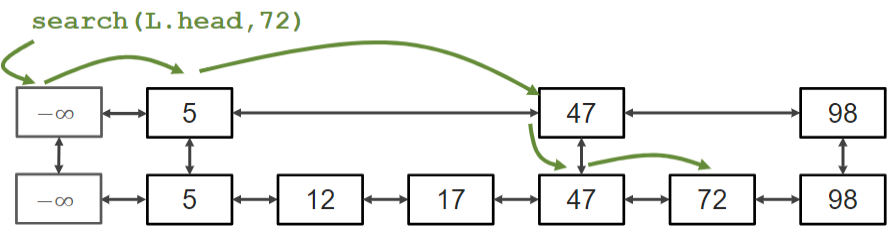
\includegraphics[width=12cm]{pictures/skiplistSuche.PNG}
                \item Verbesserung: Zusätzliche Stufen an Express-Listen 
                \item Anwendung: 
                \begin{itemize}
                    \item Gut für parallele Verarbeitung z.B. Multicore-Systeme (Einfügen und Löschen)
                    \item Dafür logarithmische Laufzeit nur im Durchschnitt
                \end{itemize}
                \item Auswahl von Elementen:
                    \begin{itemize}
                        \item Abhängig von einer gewählten Wahrscheinlichkeit $p$ 
                        \item Element kommt mit Wahrscheinlichkeit $p$ in übergeordnete Liste
                        \item Höhe: $h = O(log_{\frac{1}{p}}n)$
                        \item Anzahl Elemente: $n \Rightarrow pn \Rightarrow p^2n \Rightarrow ...$ (unten nach oben)
                    \end{itemize}
            \end{itemize}

        \item \fatsf{Implementierung}
            \begin{itemize}
                \item[]
                        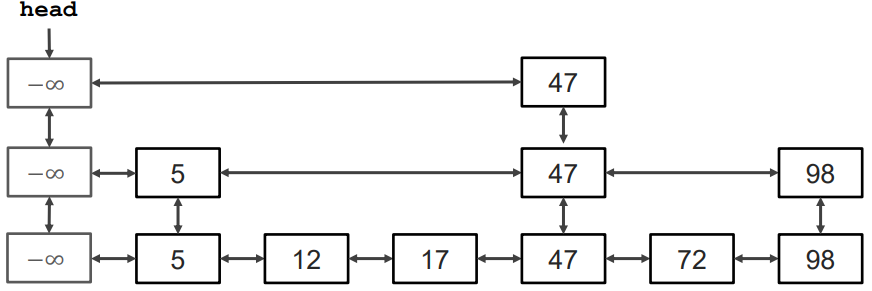
\includegraphics[width=12cm]{pictures/skiplistImplement1.PNG}\\
                        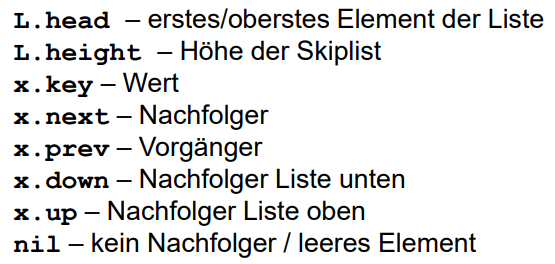
\includegraphics[width=8cm]{pictures/skiplistImplement2.PNG}
            \end{itemize}
\clearpage
        \item \fatsf{Suche}
            \begin{itemize}
                \item Laufzeit ist von Expresslisten abhängig
                \item[]
                    \begin{ccode}[autogobble]{title={search(L, k)}}
                    current = L.head;
                    WHILE current != nil DO
                        IF current.key == k THEN 
                            return current;
                        IF current.next != nil AND current.next.key <= k THEN
                            current = current.next;
                        ELSE
                            current = current.down;
                    return nil;
                    \end{ccode}
            \end{itemize}

        \item \fatsf{Einfügen}
            \begin{itemize}
                \item Füge auf unterster Ebene ein
                \item Evtl. auf höheren Ebenen mit zufälliger Wahl mithilfe von $p$ auf jeder Ebene
            \end{itemize}

        \item \fatsf{Löschen}
            \begin{itemize}
                \item Entferne Vorkommen des Elements aus allen Ebenen
            \end{itemize}
        
        \item \fatsf{Laufzeiten}
            \begin{itemize}
                \item {\makebox[2cm][l]{Einfügen: }} $\Theta(log_{\frac{1}{p}}n)$
                \item {\makebox[2cm][l]{Löschen: }} $\Theta(log_{\frac{1}{p}}n)$
                \item {\makebox[2cm][l]{Suchen: }} $\Theta(log_{\frac{1}{p}}n)$
                \item (Im Durchschnitt)
                \item $O$-Notation versteckt konstanten Faktor $\frac{1}{p}$
                \item Speicherbedarf im Durchschnitt: $\frac{n}{1-p}$
            \end{itemize}
    \end{itemize}
\clearpage
\subsection{Hashtables}\label{Hashtables}
    \begin{itemize}
        \item \fatsf{Idee}
            \begin{itemize}
                \item[]
                    \begin{minipage}{0.4\textwidth}
                        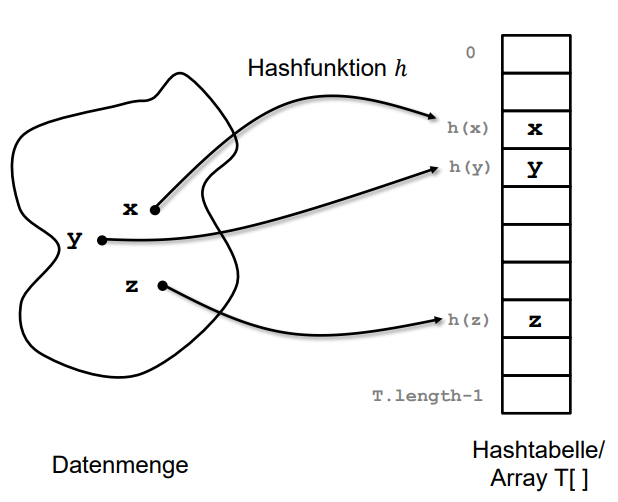
\includegraphics[width=5cm]{pictures/hashtableIdee.PNG}
                    \end{minipage}
                    \begin{minipage}{0.5\textwidth}
                        \begin{itemize}
                            \item Hashfunktion sollte gut verteilen
                            \item $h(x)$ sollte uniform sein
                            \item Unabhängig im Intervall $[0, T.length-1]$ verteilt
                            \item Einfügen mit konstant vielen Array-Operationen
                        \end{itemize}
                    \end{minipage}
                \item[]
                \item[]
                \item[]
                    \begin{minipage}{0.4\textwidth}
                        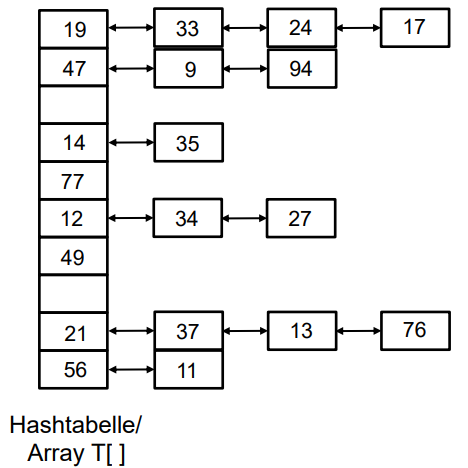
\includegraphics[width=5cm]{pictures/hashtableLinkedList.PNG}
                    \end{minipage}
                    \begin{minipage}{0.5\textwidth}
                        \begin{itemize}
                            \item Kollisionsauflösung z.B. mithilfe von LinkedLists
                            \item Neue Elemente werden vorne angefügt
                            \item Konstante Anzahl an Array-Operationen
                            \item Soviele Schritte wie die Liste lang ist 
                            \item Uniforme Hashfunktion
                            \item[] $\Rightarrow$ $\frac{n}{T.length}$ Einträge pro Liste
                        \end{itemize}
                    \end{minipage}
                \item[]
            \end{itemize}

        \item \fatsf{Hash-Funktionen}
            \begin{itemize}
                \item Universelle Hash-Funktion:
                    \begin{itemize}
                        \item Wähle zufällige $a,b \in [0, p - 1]$, $p~prim$, $a \neq 0$
                        \item $h_{a,b}(x)= ((a \cdot x + b)~mod~p)~mod~T.length$
                    \end{itemize}
                \item Krypthographische Hash-Funktionen:
                    \begin{itemize}
                        \item MD5, SHA-1, SHA-2, SHA-3
                        \item $h(x) = MD5(x)~mod~T.length$
                    \end{itemize}
            \end{itemize}

\pagebreak
        
        \item \fatsf{Hashtables vs. Bäume}
            \begin{itemize}
                \item Hashtables:
                    \begin{itemize}
                        \item nur Suche nach bestimmten Wert möglich
                        \item meist größer als zu erwartende Anzahl Einträge
                    \end{itemize}
                \item Bäume:
                    \begin{itemize}
                        \item schnelles Traversieren zu Nachbarn möglich
                        \item Bereichssuche möglich
                    \end{itemize}
            \end{itemize}
        
        \item \fatsf{Laufzeiten}
            \begin{itemize}
                \item Wählt mal $T.length = n$ ergibt sich konstante Laufzeit
                \item {\makebox[2cm][l]{Einfügen: }} $\Theta(1)$
                \item {\makebox[2cm][l]{Löschen: }} $\Theta(1)$
                \item {\makebox[2cm][l]{Suchen: }} $\Theta(1)$
                \item (Im Durchschnitt, beim Einfügen sogar im Worst-Case)
                \item Speicherbedarf i.d.R. höher als n, meist ca. $1,33 \cdot n$
            \end{itemize}
    \end{itemize}

\subsection{Bloom-Filter}\label{Bloom-Filter}
    \begin{itemize}
        \item \fatsf{Idee}
            \begin{itemize}
                \item Speicherschonende Wörterbucher mit kleinem Fehler
                \item z.B. Vermeidung von schlechten Passwörtern 
                    \begin{enumerate}
                        \item Abspeichern aller schlechten Passwörter in kompakter Form
                        \item Prüfe, ob eingegebenes Passwort im Bloom-Filter
                    \end{enumerate}
                \item z.B. Erkennen von schädlichen Websites (Chrome früher)
            \end{itemize}

        \item \fatsf{Erstellen}
            \begin{itemize}
                \item $n$ Elemente $x_0,...,x_{n-1}$
                \item $m$ Bits-Speicher z.B. als Bit-Array
                \item $k$ gute Hash-Funktionen $H_0,...,H_{k-1}$ mit Bildbereich $0,1,...,m-1$
                \item Empfohlene Wahl: $k = \frac{m}{n} \cdot ln2$ (Fehlerrate von ca. $2^{-k}$)
                \clearpage
                \item Code:
                \item[]
                    \begin{ccode}[autogobble]{title={initBloom(X, BF, H) // H Array of hash functions}}
                    FOR i = 0 TO BF.length - 1 DO 
                        BF[i] = 0;
                    FOR i = 0 TO X.length - 1 DO
                        FOR j = 0 TO H.length - 1 DO
                            BF[H[j](X[i])] = 1;
                    \end{ccode}
                \item[]
                \item[1.] Initialisiere Array mit 0-Einträgen
                \item[2.] Schreibe für jedes Element in jede Bit-Position $H_0(x_i),...,H_{k-1}(x_i)$ eine 1 
                \item[] 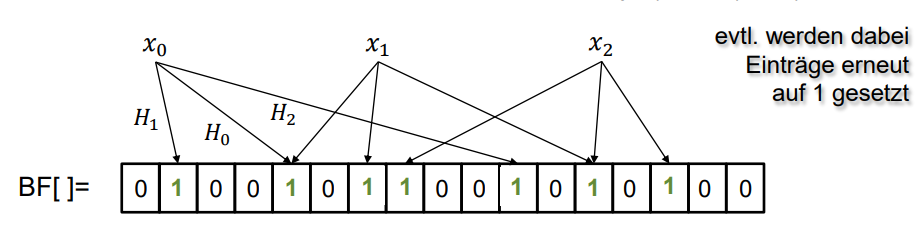
\includegraphics[width=15cm]{pictures/bloomCreate.PNG} 
            \end{itemize}

        \item \fatsf{Suche}
            \begin{itemize}
                \item[]
                    \begin{ccode}[autogobble]{title={searchBloom(BF, H, y)}}
                    result = 1;
                    FOR j = 0 TO H.length - 1 DO
                        result = result AND BF[H[j](y)];
                    return result;
                    \end{ccode}
                \item[]
                \item Gibt an, dass $y$ im Wörterbuch, falls alle $k$ Einträge für $y$ in $BF=1$ sind
                \item[] 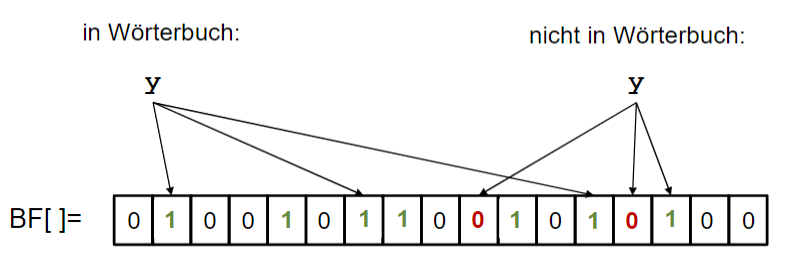
\includegraphics[width=13.5cm]{pictures/bloomSearch.PNG}
                \item Eventuell \string"false positives\string" (1, obwohl $y$ nicht im Wörterbuch)
                    \begin{itemize}
                        \item Passiert, falls die Einträge vorher von anderen Werten getroffen wurden
                        \item Daher gute Hashfunktionen und Filtergrö\ss e nicht zu klein
                    \end{itemize}
            \end{itemize}
    \end{itemize}
    \clearpage
\end{document}
